% !TEX root = 0_main.tex
\chapter{Garbled Processor}\label{chap:processor}
Supporting sequential circuits in the GC protocol enables us to securely evaluate a general processor as function in two-party SFE.
A processor itself receives a function (more pressingly the compiled binary code of a function) and data in its memory, then computes the function and writes the result back in the memory.
In this chapter first, we explain the problem of Private Function SFE (PF-SFE) and how a processor can solve it with limited resources.
Next, we explain how we used MIPS processor, a simple text-book processor, to solve PF-SFE problem.
Next, we study how a garbled processor can be modified to used for SFE problem as a mean to make it easy for user to develop SFE application.
Then, we explain how ARM, a more sophisticated processor, can be well suited for solving SFE development if SkipGate algorithm is applied during garbling/evaluating its circuit.

\section{Private Function Evaluation}\label{sec:processor-pfsfe}
Two-party Private Function SFE (PF-SFE) allows secure computation of a function $f_{Alice}(\cdot)$ held by one party (Alice) operating on another party's data $x_{Bob}$ (Bob) while both the data and the function are kept private.
This is in contrast to the usual setting of SFE where the function is known by both parties.
PF-SFE is especially useful when the function is proprietary or classified.

It is well known that PF-SFE can be reduced to regular SFE by securely evaluating a Universal Circuit (UC) \cite{sander1999non}.
UC is a Boolean circuit capable of simulating any Boolean circuit (function) $f(\cdot)$ given the description of $f(\cdot)$ as input \cite{valiant1976universal,kolesnikov2008practical}:
$$UC(f_{Alice}(\cdot),x_{Bob}) = f_{Alice}(x_{Bob}).$$
Secure evaluation of UC completely hides the functionality of Boolean circuit of $f(\cdot)$, including its topology.
Subsequent works have shown how to allow PF-SFE while avoiding the overhead of UCs \cite{katz2011constant, mohassel2013hide}.

A UC is similar to a Universal Turing Machine (UTM) \cite{turing1936computable,herken1995universal} that receives a Turing machine description $f_{Alice}(\cdot)$ and applies it to the input data ($x_{Bob}$) on its tape \cite{davis2001engines}.
One party provides the machine description and the other one provides the initial data.
The output $f_{Alice}(x_{Bob})$ resides on the tape after the operation is completed.
A general purpose processor is a special realization of a UTM.
It receives a list of \emph{instructions} $f_{Alice}(\cdot)$ (the compiled binary code of $f_{Alice}(\cdot)$) and applies them to the input data $x_{Bob}$.

\subsection{Arithmetic Logic Unit}\label{ssec:processor-alu}
The core of conventional processors is the Arithmetic Logic Unit (ALU) which receives two \emph{operands} and an \emph{opcode} indicating the desired operation.
ALU supports an operation set consisting of operations like addition, multiplication, XOR, etc.
The ALU circuit consists of multiple sub-circuits for these operations and a MUX which selects one of their outputs.
Secure evaluation of an ALU, where the opcode comes from one party and operands come from the other party, keeps the operations private.
Thus, ALU can be thought of as an emulator of a simple UC in which the input function $f_{Alice}(\cdot)$ is limited to a single operation.

One can combine a number of ALUs to make a more comprehensive UC that can support functions consisting of multiple operations.
Unfortunately, this approach is not practical as the complexity of the circuit grows linearly with the number of operations.
On the other hand, in conventional processors, ALUs are combined with arrays of FFs, a.k.a., \emph{registers}, in order to store the intermediate values for supporting functions with arbitrarily large number of operations.
Since none of the earlier implementations of GC explicitly supported memory elements such as FFs, the ways to connect the feedback loop around the ALU were rather limited.
However, an explicit sequential description supported by TinyGarble allows us to leverage conventional processor architectures.
Therefore, the TinyGarble methodology not only provides a powerful method for generating compact circuits with a low overhead for SFE, but also paves the way for systematically building scalable sequential circuits that can be used for PF-SFE.

The idea of using an ALU or a \emph{universal next-instruction circuit} in the GC protocol can also be found in \cite{liu2014automating}.
The objective of that work was improving efficiency of SFE where the function is known by both parties, unlike PF-SFE where the function is private.
Nonetheless, instead of ALU they eventually decided to use an \emph{instruction-specific circuit} which leaks information about the function but results in less effort for non-private function evaluation.

\subsection{Memory}\label{ssec:processor-mem}
The processor accesses the memory while executing an instruction to read the instruction and data and write the data back.
If the memory is securely evaluated along with the processor, the access patterns must be also oblivious to both parties.
On the other hand, if the memory is not evaluated securely, the access patterns could be revealed that in turn could reveal information about the function to Bob and about the data to Alice.
For example, the instruction read pattern discloses the branching decisions in the function which may leak information about the data.
Because of TinyGarble sequential methodology, the memory can be easily implemented using MUX and arrays of FFs.
Thus, it can be included in the processor circuit to be evaluated securely using the GC protocol.
However, inclusion of MUXs and FFs increases the operation time and communication linearly with respect to the memory size.

One alternative approach for hiding memory access patterns is the use of Oblivious Random-Access Machine (ORAM) protocols \cite{goldreich1996software} which allows oblivious load/store operations with amortized poly-logarithmic overhead at the expense of increasing the round complexity of the GC protocol \cite{gordon2012secure,liu2014automating,lu2013garble,gentry2014garbled}.
For the sake of simplicity, we do not use ORAM in this work.
However, one can simply connect our implementation of PF-SFE to an ORAM to benefit from its lower amortized complexity.
As another alternate, \cite{zahur2013circuit} showed that algorithms can sometimes be rewritten to use data structures such as stacks, queues, or associative maps for which they give compact circuit constructions of poly-logarithmic size.

\section{Garbled Processor for PF-SFE}\label{sec:processor-pro-pfsfe}
\subsection{Global flow}\label{ssec:processor-mips-flow}
We assume Alice provides the private function $f_{Alice}(\cdot)$ and Bob provides private data~$x_{Bob}$.
At the end of the operation, only Bob learns the output $f_{Alice}(x_{Bob})$.
Note that we are not considering the case where both parties learn the output as that would allow Alice to learn Bob's private data with an identity function ($f\equiv I$).
The protocol is as follows:

\begin{enumerate}
\item
  Alice and Bob agree on an instruction set architecture (ISA), its implementation (i.e., the processor circuit), the maximum number of sequential cycles, and the configuration of data $x_{Bob}$ in the memory.
\item
  Alice compiles the function $f_{Alice}(\cdot)$ according to the ISA.
  Her input is the compiled binary of the function.
\item
  Bob prepares his input based on the agreed configuration to initialize the processor memory.
\item
  Using any secure GC framework, Alice garbles the processor circuit for the maximum number of sequential cycles and Bob, after receiving his inputs with OT, evaluates the garbled processor circuit for the same number of cycles.

\item
  Alice reveals the output types such that Bob learns the value of the output $f_{Alice}(x_{Bob})$ stored in memory.
  This needs to be done only for agreed memory locations containing the outputs such that Bob does not learn intermediate values in the memory.
\end{enumerate}

Because of secure evaluation using the GC protocol in Step 4, no information about values in the circuit will be leaked except the output.
Without knowing internal values in the processor circuit, none of the parties can distinguish instructions or memory access patterns.
In the following, we demonstrate an implementation of a processor supporting the MIPS (Microprocessor without Interlocked Pipeline Stages) ISA, as an example of a garbled processor for securely evaluating private functions.

\subsection{MIPS}\label{ssec:processor-mips}
MIPS is a text-book Reduced Instruction Set Computing (RISC) ISA \cite{kane1992mips}.
The RISC ISA consists of a small set of simplified assembly instructions in contrast to Complex Instruction Set Computing (CISC) (e.g., x86 ISA) which includes more complex multi-step instructions \cite{hennessy2012computer}.
We choose a RISC ISA processor instead of CISC for the following main reasons: (i) lower number of non-XOR gates, (ii) simple and straightforward implementation, and (iii) availability and diversity of open-source implementations.
Moreover, we choose a single-cycle MIPS architecture (i.e., one instruction per sequential cycle).
Other architectures (i.e, multi-cycle and pipelined) increase the performance of the processor by parallelization.
However, the GC protocol does not benefit from such low level parallelization.
The only important factor for GC is the total number of non-XORs which is smaller in the single-cycle MIPS.
We follow the Harvard Architecture which has distinct instruction memory (IM) and \acrfull{dm} in order to separate the parties' inputs.
IM is a Read-Only Memory (ROM) that stores Alice's instructions.
DM is a Random Access Memory (RAM) that is initialized with Bob's input.
The parties' inputs are connected to the initial signal inputs of FFs in the memories.
Bob's outputs are connected to the outputs of FFs in the specified address of DM.
The output address in DM is part of the agreed memory configuration.

\begin{figure}[ht]
\centering
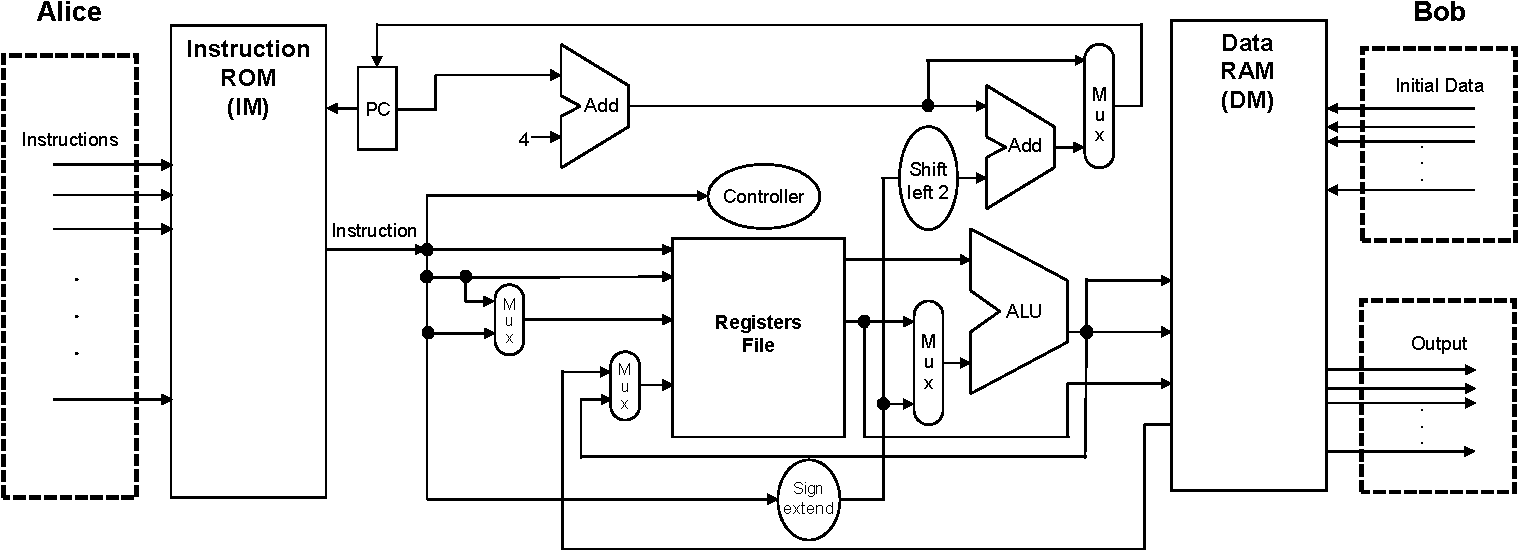
\includegraphics[width=0.95\textwidth]{mips-complex-crop.pdf}
\caption{Lite MIPS architecture.
  Alice's and Bob's inputs and the output are shown.}\label{figure:mips}
\end{figure}

\fig{figure:mips} shows the overall architecture of our 32-bit MIPS processor.
It is based on the Plasma project in opencores \cite{rhoads2006plasma}.
We modified the circuit such that the instruction ROM (IM) and the data RAM (DM) are separated.
The original Plasma processor supports all the MIPS~I ISA except unaligned memory access.
In our implementation, we also omit division instructions because of their large overhead.
Any arbitrary C/C++ function can be easily compiled to MIPS~I assembly code using a cross-platform compiler e.g., GNU gcc.

In 32-bit MIPS, the program counter (\emph{PC}) is a 32-bit register (array of FFs) that points to the instruction being executed at the current cycle.
The instruction is fetched from IM based on the current PC value.
The \emph{controller} unit is responsible for setting signals to perform the instruction.
In 32-bit MIPS, the \emph{register file} consists of 32 registers of 32-bit each.
In each cycle, at most two registers can be read and at most one register can be written back.
ALU receives the read register(s) or a sign extended \emph{immediate} as operands.
ALU also receives an opcode from the controller unit.
The output of ALU will be either written back to the register file or fed to DM as an address for load/store.
The loaded data from DM is written back to the register file.
In each cycle, PC is incremented by 4 to point to the next instruction in IM or is changed according to a branch or jump instruction.

\section{Garbled Processor for SFE}\label{sec:processor-mips-sfe}
In the previous section we discuss the idea of garbling a processor as a solution for hiding the function in PF-SFE.
Besides enabling PF-SFE, another advantage of a garbled processor is usability for non-expert users since it can be programmed using high-level languages, whereas other frameworks for the GC protocol require tedious Boolean circuit construction.
However, garbling and evaluating the entire processor incurs a tremendous cost compared to SFE solutions due to stronger privacy requirements in PF-SFE.

In this section, we expand the garbled processor introduced in \section{sec:processor-pro-pfsfe} and introduce a framework for secure computation that provides scalable support for generalized SFE.
The framework provides theres options: a high performance with a relaxed privacy setting, the more security-demanding PF-SFE with higher cost (similar to the one in \sect{sec:processor-pro-pfsfe}), and a flavor in-between.

To avoid information leakage about the function (i.e., PF-SFE), we employ the MIPS circuit with its full Instruction Set (IS), which incurs a large overhead due to garbling and evaluating of the entire IS.
We can also compile the function using only a subset of the IS: restricted IS (i.e., semi-private function).
A third alternative is public function mode in which the function is compiled using only an application-specific subset of the IS that is required for executing the function.
In the following, we discuss these modes of function evaluation and the trade-off between privacy and performance further.

\subsection{Garbled Processor for Public Functions}\label{ssec:processor-mips-sfe-public}
Using a general-purpose processor with its entire IS in SFE results in garbling a large processor which is very costly and unnecessary since both parties know the function instructions being executed but not their results.
Hence, garbling a limited application-specific IS for executing each instruction is sufficient to achieve privacy.
To further reduce the IS, assuming for example, a function that consists of \numprint{10} instructions, we could theoretically generate $2^{10} -1$ netlists (netlists of IS with different combinations of the 10 instructions, excluding the netlist with zero instructions).
At run-time, one of these netlists is plugged in (garbled and evaluated) at each instruction step depending on the expected instructions.
However, to make it more reasonable (generate fewer netlists), for functions with control flow independent of private data, we know in advance which instruction will be executed at each step.
Thus, we need only the netlist of the processor implementing IS with that specific instruction, restricting the required netlists in this case to \numprint{10}.
For functions with control flow dependent on private data, a simple static analysis can be used to specify the combination of possible instructions at each step, and hence the required IS netlist as proposed in \cite{wang2016secure}.

\subsection{Garbled Processor for Semi-Private Functions}\label{ssec:processor-mips-sfe-semiprivate}
The main cost for garbling a processor with its entire IS results from garbling circuits for expensive instructions like multiplication and division.
Most compilers are able to avoid these costly instructions and replace them with cheaper loops of shifts, addition, and subtraction instructions.
This would eliminate the need for the Mult/Div unit in the processor and reduce the cost of garbling per instruction on one hand.
However on the other hand, one expensive instruction will be replaced with multiple cheap instructions, thus increasing the total number of instructions.
For example, multiplying two 32-bit numbers with the MULT instruction in MIPS requires \numprint{15} cycles and a circuit of \numprint{13257} non-XOR gates\footnote{XOR gates are evaluated freely in GC according to the free-XOR optimization of \cite{kolesnikov2008improved}.}, while it requires at least \numprint{31} cycles and a circuit of \numprint{9,676} non-XOR gates when using a conditional loop over an ADD instruction.
We call this mode ``semi-private'' since it only reveals partial information about instructions used in the program (that the program does not use division/multiplication) and increases the probability of guessing an instruction by reducing the subset of possible instructions (restricted IS).

\subsection{Garbled Processor for Private Functions}\label{ssec:processor-mips-sfe-private}
In the standard 2-party PF-SFE, Alice provides the function $f_{Alice}(\cdot)$ and Bob provides the input data $x_{Bob}$ and the output is $f_{Alice}(x_{Bob})$.
Similar to \sect{sec:processor-pro-pfsfe}, the garbled processor receives a list of \emph{instructions} of compiled $f_{Alice}(\cdot)$ and applies them to the input data $x_{Bob}$ in memory and the output will be written back to the memory.
To avoid information leakage about the private function, we use a general-purpose processor with its entire IS (full IS).

\section{Hardware Implementation of Garbled Processor}\label{sec:processor-hardware}
To the best of our knowledge, the fastest implementation of GC in hardware was~\cite{jarvinen2010garbled}.
However, their performance is much slower than software implementation such as JustGarble~\cite{bellare2013efficient}.
This is because JustGarble utilizes a more efficient fixed-key AES for garbling instead of an expensive hash function.
Thus, it is possible that a hardware implementation leveraging the latest GC optimizations including fixed-key AES garbling would outperform the software implementation.
Furthermore, a processor is essentially a sequential circuit and its evaluation requires sequential GC which no hardware implementation of GC supports.

Our GC evaluator is based on the most recent optimizations listed in \sect{ssec:prelim-imp}.
Its architecture is shown in \fig{fig:evaluator} and consists of:
(1) Sequential Simple Circuit Description (SSCD) memory: read-only memory that stores the information about gates in the MIPS circuit in SSCD format (see \appx{sec:engine-sscd})
(2) GC Label memory: read-write random-access memory that stores GC ciphertext labels of all wires in the corresponding MIPS circuit.
(3) Garbled Tables (GT) memory: read-write random-access memory that stores the ciphertext garbled tables of each non-XOR gate in the MIPS circuit that are generated by Alice (garbler).
(4) Sequential Handler: controller that supports evaluation of the sequential circuits with the GC protocol.
(5) Evaluator Engine: main functionality of GC evaluation according to Yao's GC protocol and its most recent optimizations \cite{kolesnikov2008improved, bellare2013efficient, zahur2015two, songhori2015tinygarble}.

As shown in \fig{fig:evaluator}, Bob's input labels in the Label memory are initialized by the OT protocol with Alice.
The rest of the labels in the Labels memory and the Garbled Tables memory are received in clear-text from Alice.

\begin{figure}
\centering
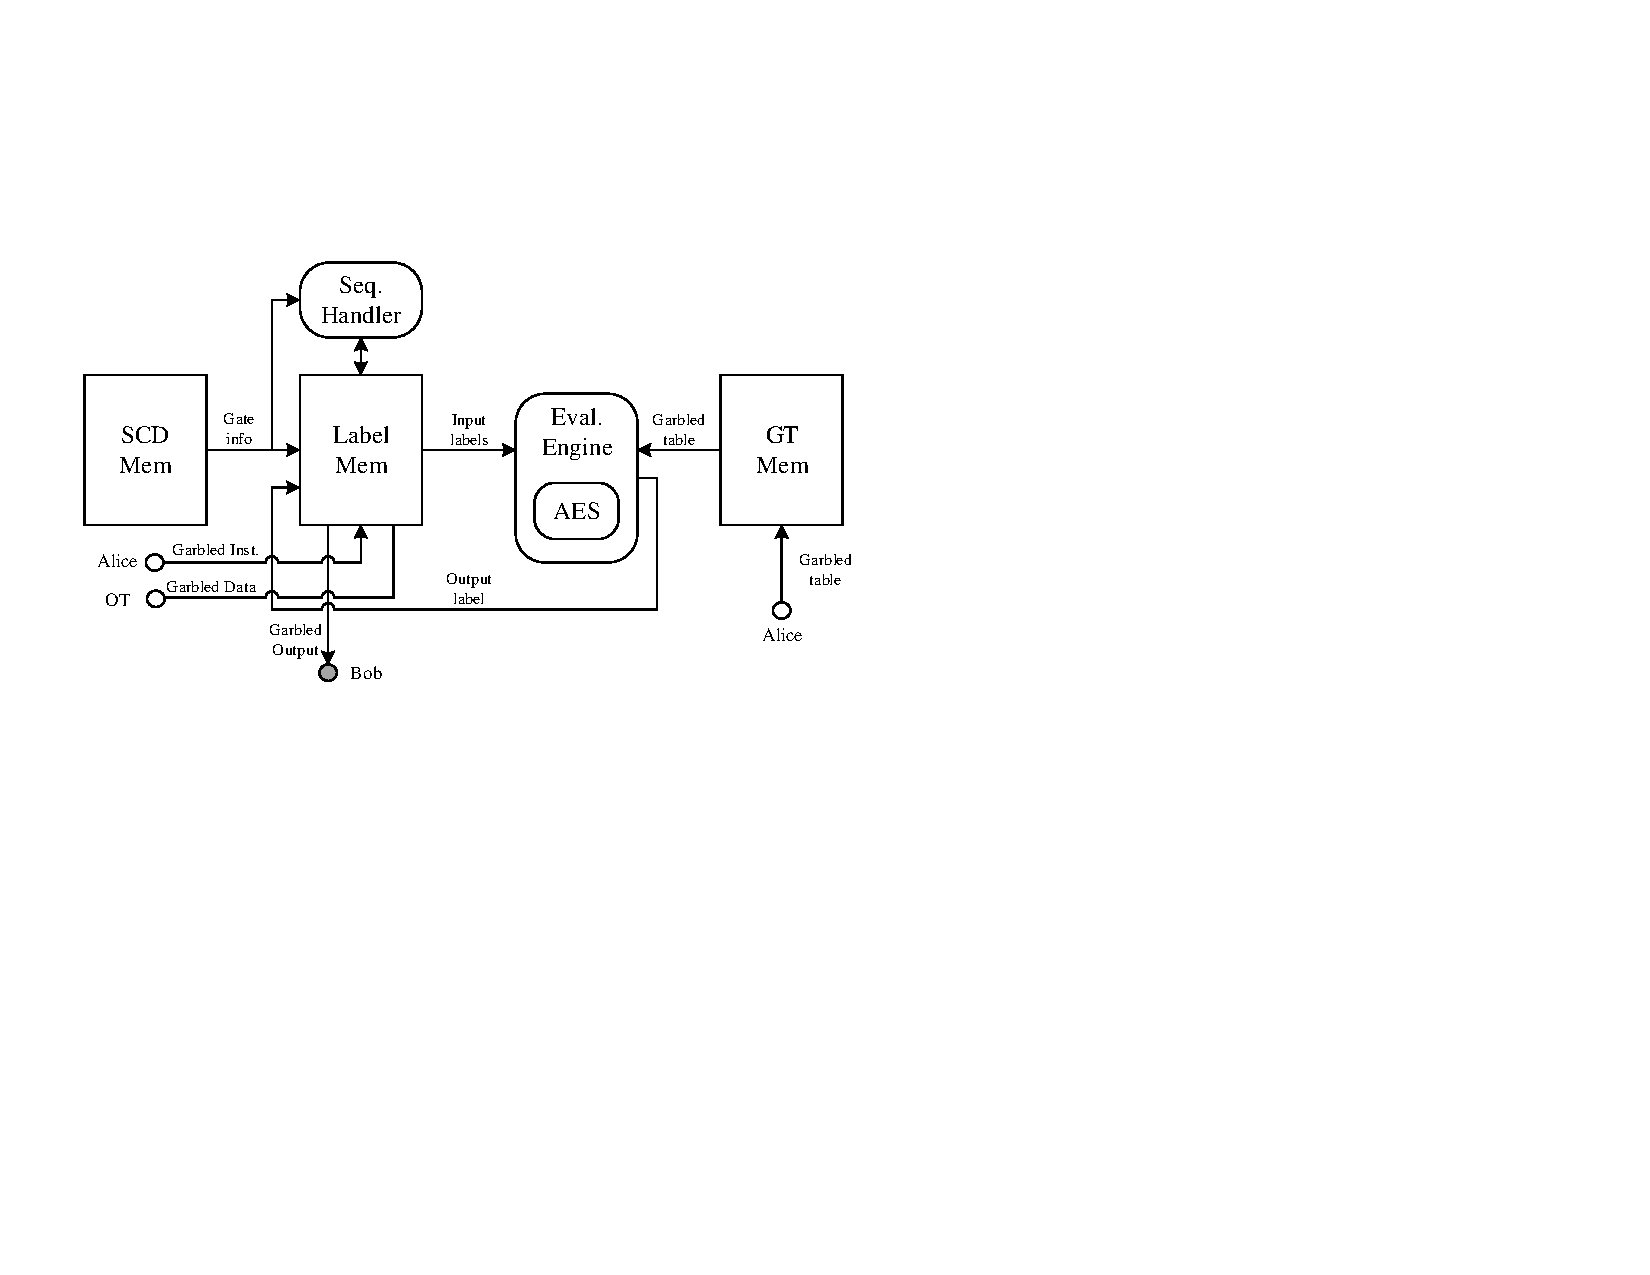
\includegraphics[width=\textwidth]{Evaluator-crop.pdf}
\caption{Our GC Evaluator Architecture.}
\label{fig:evaluator}
\end{figure}

\subsubsection{Pipelined Evaluator Engine and Gate Dependency}\label{ssec:processor-hardware-pipeline}
To maximize the performance of the GC evaluator, we use a 20-stage pipelined AES implementation \cite{hsing2013tiny} inside our Evaluator Engine module. It increases the throughput of the module by increasing the maximum operating clock frequency of the engine. We also add one stage for the rest of the GC evaluation functionality.

Due to the free-XOR technique \cite{kolesnikov2008improved}, evaluating an XOR gate requires only XOR-ing the input labels while evaluating a non-XOR gate requires two AES encryptions (due to half-gates technique presented in \sect{ssect:gc}, and was one encryption before). Therefore, evaluation of an XOR gate can be done in only one stage of the AES pipeline. Different timing for XOR and non-XOR gates introduces a challenge for handling dependencies of gates' inputs and output. A gate cannot enter the evaluation pipeline if its inputs are another gate's output which is not yet evaluated. This results in pipeline stalls which degrade the overall performance. To mitigate this, we push XOR gates to the latest empty stage of the pipeline such that the subsequent dependent gates can enter the pipeline as soon as possible.

\subsection{Hardware Prototype Challenges}\label{ssect:challenges}
We only use on-chip memory for our proof-of-concept in this work. However, this prototype can be extended to support interfacing with off-chip memory which would store garbled tables and labels of larger garbled processor circuits and functions. It can also interface with another FPGA emulator of the garbler which generates the garbled tables and labels and streams them to our evaluator. A wide range of scenarios are now feasible owing to our current hardware platform and state-of-the-art optimized GC evaluator.
%
Such extensions would incur additional area and performance overheads, but would allow upscaling of our implementation to support garbled processor circuits and benchmarks in the Gigabytes range. We emphasize that we provide in this work a proof-of-concept prototype to motivate further research in this direction to bring garbled processors some steps closer to the realm of feasible practical implementations.

\section{ARM2GC: Garbled ARM for SFE}
In this section, we present ARM2GC, a GC framework based on a garbled ARM processor and the SkipGate algorithm.
The framework aims to simplify the development of privacy-preserving applications while keeping the garbling cost as low as the best optimized garbled circuits.
We first describe the overview of ARM2GC and its API for GC development.
Then, we explain how ARM's unique architecture helps to decrease garbling overhead.
Next, the effect of SkipGate in reducing the garbling cost is discussed.
Finally, we discuss why we do not employ Oblivious RAM for ARM2GC.

\subsection{Global Flow}\label{ssec:arm-global}
The ARM2GC framework allows users to write two-party SFE program in C/C++ (or any language that can be compiled to ARM binary code).
\fig{fig:frwk_overview} shows the overview of the framework.
The SFE program is compiled using an ARM cross-compiler, e.g., gcc-arm-linux-gnueabi.
The compiled binary code and the synthesized ARM processor circuit are fed to the SkipGate algorithm as the public input $p$ and the Boolean circuit, respectively.

\begin{figure}[ht]
\centering
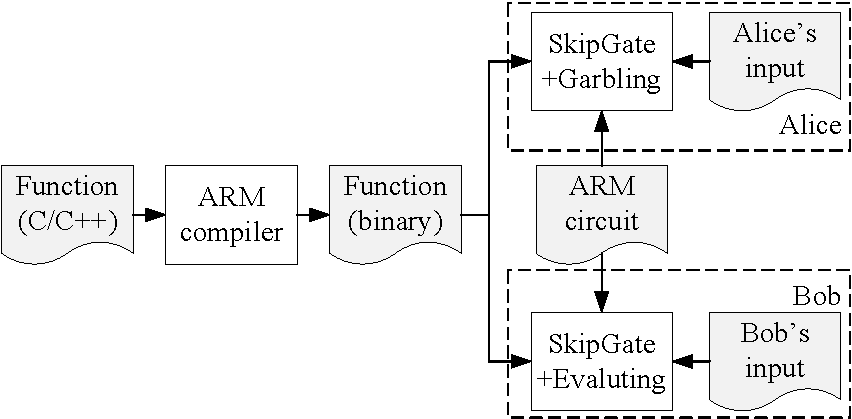
\includegraphics[width=0.45\textwidth]{frwk_overview-crop.pdf}
\caption{Overview of the ARM2GC framework.}\label{fig:frwk_overview}
\end{figure}

The ARM2GC framework supports the following API:
\begin{lstlisting}[language=C,basicstyle=\ttfamily,keywordstyle=\color{blue}\ttfamily,stringstyle=\color{red}\ttfamily,commentstyle=\color{CommentColor}\ttfamily]
void gc_main(
  const int *a,// Alice's input
  const int *b,// Bob's input
  int *c) {// output array
  // The user's code goes here.
}
\end{lstlisting}

The entry function, \texttt{gc\_main}, receives three arguments: pointers to Alice's input, Bob's input, and the output.
The framework has five separate memory elements (consisting of flip-flops and MUXs) to store: Alice's inputs, Bob's inputs, output, stack, and instructions.
The flip-flops in the instruction memory are initialized with the compiled binary code that is known to both parties (the public input $p$).
The flip-flops in Alice's and Bob's memories are initialized with labels corresponding to their private inputs $a$ and $b$ respectively.
The other flip-flops in the stack, output, pipeline registers, and the register file are initialized to zero.
The ARM circuit is garbled using sequential garbling process~\cite{songhori2015tinygarble} for a pre-specified number of clock cycles $cc$.

A signal called \textit{terminate} is produced by the ARM circuit that indicates if \texttt{gc\_main} function is returned.
The signal can be revealed to the parties once in $T$ cycles (predetermined by parties) to reduce the total number of cycles for garbling.
For $T=1$, the parties instantly identify the termination, but the exact number of cycles the function evaluated for the given inputs is revealed.
A larger $T$ would reduce this information leakage, but increase the garbling cost.
Eventually, when the function is executed, the parties reveal the content of the output memory to each other.
Appendix \ref{sec:engine} provides more details about the support of the terminate signal support in TinyGarble GC engine.

\subsection{ARM as a Garbled Processor}\label{ssec:arm}
In this work, we choose ARM as our garbled processor which is a more ubiquitous and sophisticated processor compared to MIPS~\cite{songhori2015tinygarble, wang2016secure, songhori2016garbledcpu}.
ARM has two main advantages:
(1) Pervasiveness: the compilers and tool-sets of ARM are under constant scrutiny, updating, and probably, more optimized as a result.
(2) Conditional Execution: Designed to improve performance and code density, conditional execution in ARM allows each instruction to be executed only if a specific condition is satisfied~\cite{sloss2004arm}.

ARM compilers tend to replace conditional branches with conditional instructions to make the flow of the program predictable, and thus, lower the cost of branch mis-prediction.
Similarly, in garbled processor, the main design effort is to make sure that the flow of the program is predictable so that the next instruction remains public.
Replacing conditional branches with conditional instructions in garbled ARM generates a code with a predictable flow.
\fig{fig:conditional_exec} shows an example function compiled into assembly with and without the conditional execution.
Moreover, we modify the ARM controller such that conditional instructions always take the same number of cycles regardless of their condition (taken or not taken). Otherwise, the program flow will be dependent on the secret condition and as a result, program flow itself will become secret which in turn reduces the efficiency of the execution.

\begin{figure}[t]
    \centering
    \begin{subfigure}{0.40\columnwidth}
        \centering
        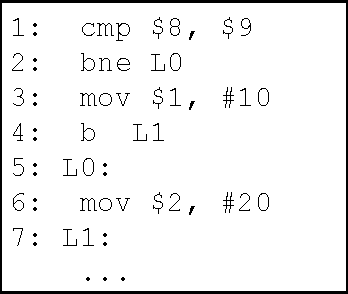
\includegraphics[width=\textwidth]{conditional_exec_wo-crop.pdf}
        \caption{Without Conditional Execution}
    \end{subfigure}
    ~
    \begin{subfigure}{0.40\columnwidth}
        \centering
        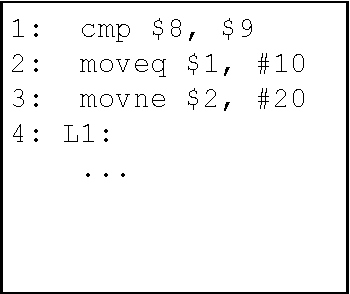
\includegraphics[width=\textwidth]{conditional_exec_w-crop.pdf}
        \caption{With Conditional Execution}
    \end{subfigure}
    \caption{An example code showing how conditional execution in ARM can reduce the code size and make the program flow predictable.}\label{fig:conditional_exec}
\end{figure}

We modify and remove a few features from the ARM processor like interrupts, co-processors, and performance-related components including cache and pipeline.
The last group does not bring any performance advantages in the GC protocol, as the circuit is garbled/evaluated gate by gate (serially).
Note that unlike in hardware, the performance of GC does not increase by parallelizing gates in the circuit.
In the GC protocol, the total number of non-XOR gates is the only factor affecting the performance, not the circuit's topology.

Implementation of ARM processor results in a complex and large netlist ($\approx 5$ times larger than MIPS processor).
Thus, using ARM instead of MIPS in the previous garbled processor approaches~\cite{wang2016secure, songhori2016garbledcpu} would incur even a higher cost.
However, majority of the components of the ARM processor remain idle during  execution of an instruction.
In the next section we describe how SkipGate utilizes this characteristic to minimize the cost of garbling the ARM processor.

\subsection{How SkipGate Helps}
As explained above, the instruction memory of the ARM processor is initialized with public values. Therefore, if the program counter (the address of the next instruction) is public, the next instruction becomes public as well.
As a result, the control path also becomes public and SkipGate can easily detect the idle components to mark them for skipping.
Moreover, due to SkipGate, the gates of the active components that are only transporting data between memory, register file, and ALU act as wires and do not incur any cost.
According to SkipGate's notation, the ARM Boolean circuit is a 3-input function $c = f(a,b,p)$ where $p$ is the public binary code and $a$ and $b$ are the parties' private inputs.
SkipGate reduces the ARM circuit into a smaller circuit of $c = f_p(a,b)$ where $f_p$ is able to perform the exact operation required in the public binary code $p$, e.g., for example $c = a + b$.
Therefore, the main garbling cost is paid only for the actual computation on the secret values.
As explained in the previous section, SkipGate performs these optimizations at the gate-level, in contrast to instruction-level of~\cite{wang2016secure, songhori2016garbledcpu}.

\subsection{Why not Sub-linear Oblivious RAM?}
As mentioned in \sect{ssec:arm-global}, we use an array of MUXs and flip-flops to implement the register file in ARM circuit.
This means that the cost of accessing the register file, when performed obliviously, is linear with respect to its size.
One natural question would be why we did not employ Oblivious RAM (ORAM) that enables oblivious access to memories in the GC protocol with sub-linear cost~\cite{wang2014scoram, zahur2016revisit}.
The reason is that, in most cases, the access to the register file is not required to be oblivious.
Since the instructions come from a publicly known instruction memory, both parties know which register of the register file is read or written.
The SkipGate algorithm utilizes this to skip garbling of the gates in the MUXs of the register file, thus, no cost is required for such accesses.
With ORAM, all the accesses to the register file would be the costly oblivious access of ORAM.

In rare occasions where two or more instructions should be garbled at a time, accessing a register would not be free using MUXs and SkipGate.
These cases only happen when ARM compiler fails to replace a conditional branch on a secret value with conditional instructions.
The user can typically alter the program in a way that the compiler avoids such branches and replaces it with conditional instructions instead.
However, in these cases, the SkipGate algorithm removes most of the gates in the register file.
Since the cost of fetching instructions remains smaller than that of break-even points of sub-linear ORAMs, using ORAM would not improve the efficiency for this case either.

\begin{figure}[h]
\centering
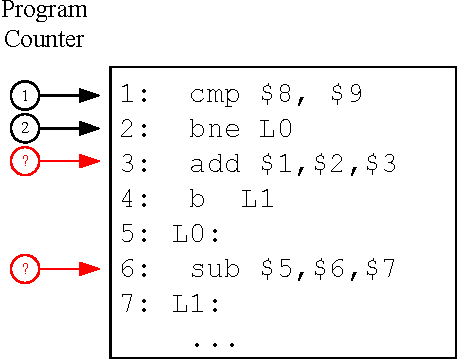
\includegraphics[width=0.60\columnwidth]{branch-crop.pdf}
\caption{In case of compiler failure to replace a secret branch with conditional instructions, the parties do not know which instruction is executed after the branch.
Thus, the instruction becomes secret.}
\label{fig:branch}
\vspace{-5pt}
\end{figure}

\fig{fig:branch} shows an example where after execution of a branch on a secret value, the next instruction becomes secret and unknown to parties.
In this example, the program counter can be either 3 or 6 depending on the outcome of the comparison in Line 1.
Thus, two instructions \texttt{add \$1, \$2, \$3} (\texttt{\$3 = \$1 + \$2}) and \texttt{sub \$5, \$6, \$7} (\texttt{\$5 = \$6 - \$7}) have to be garbled/evaluated at the same time.
For fetching the second register in instruction from the register file, we only have two choices: \texttt{\$2} and \texttt{\$6}.
This means that, instead of having a complete oblivious access to the register file with 16 choices, we only have to obliviously select between 2 of the 16 registers.
This costs far less than 1-out-of-16 oblivious access.
The cost of oblivious access using MUXs and SkipGate to a {\it subset} of a memory is equal to an oblivious access to a memory with size of the subset.

\begin{figure*}[ht]
\centering
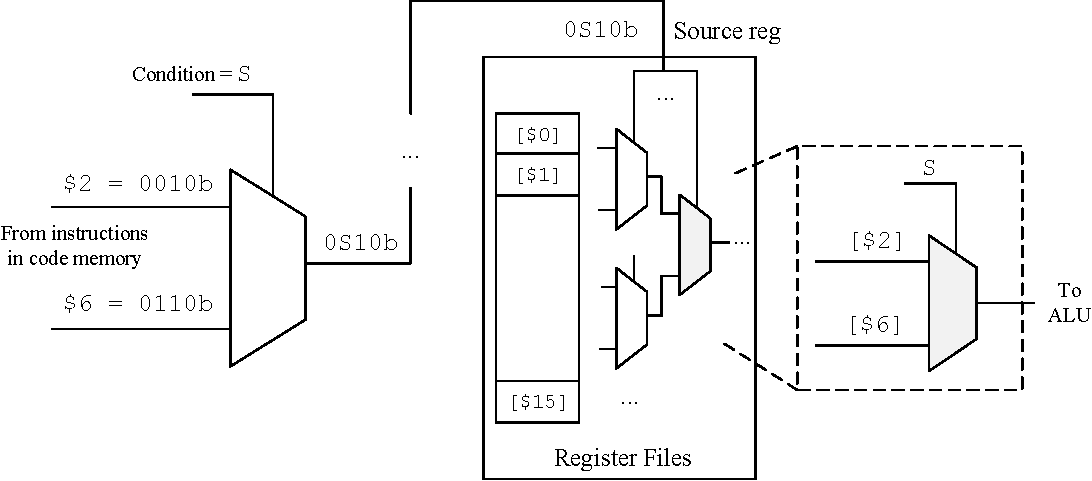
\includegraphics[width=0.65\textwidth]{registers-crop.pdf}
\caption{Bit-precise details of how source register is fetched while executing two instructions \texttt{add \$1, \$2, \$3} and \texttt{sub \$5, \$6, \$7} at the same time after a branch on a secret condition value \texttt{S}.}
\label{fig:registers}
\end{figure*}

\fig{fig:registers} illustrates the details of the above example where bit \texttt{S} is the secret bit that separates the branches of computation that each leading into a different instruction.
The address of the source register is computed by a MUX over the two options in the two instructions: MUX(\texttt{\$2, \$6, S}) = MUX(\texttt{0010b, 0110b, S}) = \texttt{0S10b}.
The most and least significant bits are, in either case, zero, and thus it will remain zero in the output.
The bit 1 is one in both cases and remains one.
The bit 2 is zero if \texttt{S==0} and is one if \texttt{S==1}, and thus this bit is equal to \texttt{S}.
Now, let us look at the MUXs in the registers files that fetch the source register.
The MUXs connected to the known bit can be evaluated separately by both parties, and thus they will be avoided by SkipGate.
Within the MUXs connected to \texttt{S}, only the one that selects between \texttt{[\$2]} and \texttt{[\$6]} remains for garbling and the rest will be removed due to non-positive fanout.

% why not ORAM for code and data memory
The rationale for using array of MUXs in the register file also applies to the code, data, and stack memories where the access is almost always public and known to both parties.
In the worst case, only a subset of memory are accessed obliviously, thus making the cost of memory access below the threshold of switching to ORAMs.
% However, when a user explicitly develops a program where a large enough array is accessed obliviously, a sub-linear ORAM~\cite{zahur2016revisit, liu2015oblivm, wang2014scoram} can be integrated as the additional memory to our framework.
% It can be done by adding an ORAM client circuit beside ARM processor and connecting the necessary wires.

% Research question
The mixture of the SkipGate algorithm and garbled processor introduces an unusual use-case for oblivious memory where oblivious access is performed only on a varying subset of the memory.
The subset can be different from one access to the other.
The current sub-linear ORAM protocols cannot address this scenario efficiently. Thus, an interesting research question is raised:

\textbf{Is it possible to \textit{obliviously} access (read/write) a varying subset of the memory with a \textit{sub-linear} cost in terms of the subset size?}
